\documentclass[pdftex,12pt,a4paper]{article}

\usepackage{graphicx}  
\usepackage[margin=2.5cm]{geometry}
\usepackage{breakcites}
\usepackage{indentfirst}
\usepackage{pgfgantt}
\usepackage{pdflscape}
\usepackage{float}
\usepackage{epsfig}
\usepackage{epstopdf}
\usepackage[cmex10]{amsmath}
\usepackage{stfloats}
\usepackage{multirow}

\renewcommand{\refname}{REFERENCES}
\linespread{1.3}

\usepackage{mathtools}
%\newcommand{\HRule}{\rule{\linewidth}{0.5mm}}
\thispagestyle{empty}
\begin{document}
\begin{titlepage}
\begin{center}
\textbf{}\\
\textbf{\Large{ISTANBUL TECHNICAL UNIVERSITY}}\\
\vspace{0.5cm}
\textbf{\Large{COMPUTER ENGINEERING DEPARTMENT}}\\
\vspace{2cm}
\textbf{\Large{BLG 222E\\ COMPUTER ORGANIZATION\\ PROJECT 1 REPORT}}\\
\vspace{2.8cm}
\begin{table}[ht]
\centering
\Large{
\begin{tabular}{lcl}
\textbf{PROJECT NO}  & : & 1 \\
\textbf{PROJECT DATE}  & : & 10.04.2023 \\
\textbf{GROUP NO}  & : & G24 \\
\end{tabular}}
\end{table}
\vspace{1cm}
\textbf{\Large{GROUP MEMBERS:}}\\
\begin{table}[ht]
\centering
\Large{
\begin{tabular}{rcl}
150200029  & : & HAVVA EDA KÖRPE \\
150200066  & : & YUSUF EMİR SEZGİN \\
150200033  & : & ÖZKAN GEZMİŞ \\
\end{tabular}}
\end{table}
\vspace{2.8cm}
\textbf{\Large{SPRING 2023}}

\end{center}

\end{titlepage}

\thispagestyle{empty}

\setcounter{tocdepth}{4}
\tableofcontents
\clearpage

\setcounter{page}{1}

\section{INTRODUCTION}
Data operations that are done with registers are called microoperations. To obtain the results of these operations Arithmetic Logic Units (ALU) are used in the CPU. In this project, we have learned the working principle of this system. Then, we used Verilog to create an ALU system and examined its process. After the implementation, using test files, the simulation has been analyzed.


\section{MATERIALS AND METHODS}
We used our Digital Design knowledge and slides that were provided by lecturers. We have provided the essential screenshots and explanations in this section.

\subsection{PART 1}
In this section, the n-bit register has been designed to use for different purposes. Outputs of the register are controlled with FunSel and Enable (E) inputs.


\begin{figure}[H]
	\centering
	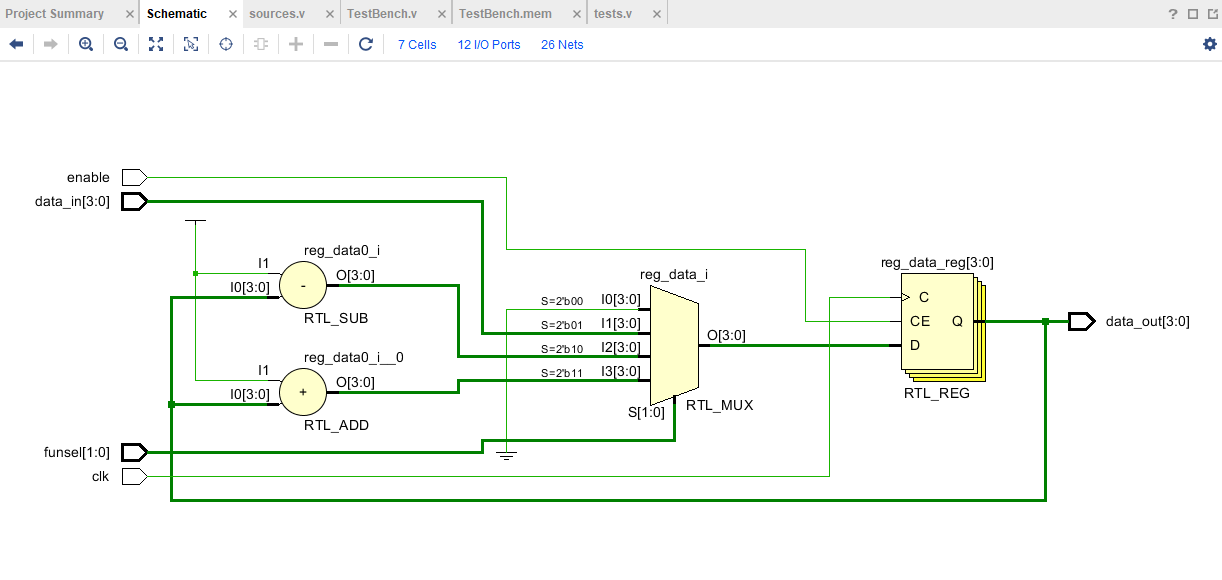
\includegraphics[width=1\textwidth]{Project1/Design Photos/nbit_register.png}	
	\caption{N-Bit Register RTL}
	\label{figone}
\end{figure}

\begin{figure}[H]
	\centering
	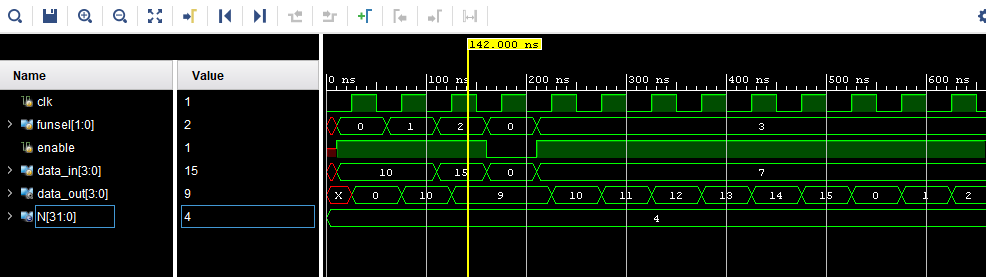
\includegraphics[width=1\textwidth]{Project1/Test Photos/nbit_register_test.png}	
	\caption{N-Bit Register Simulation}
	\label{figtwo}
\end{figure}

\subsection{PART 2}


\subsubsection{PART 2.A}
Instruction register (IR) using additional low/high signal that indicates the Most Significant and Least Significant bits have been created. 

\begin{figure}[H]
	\centering
	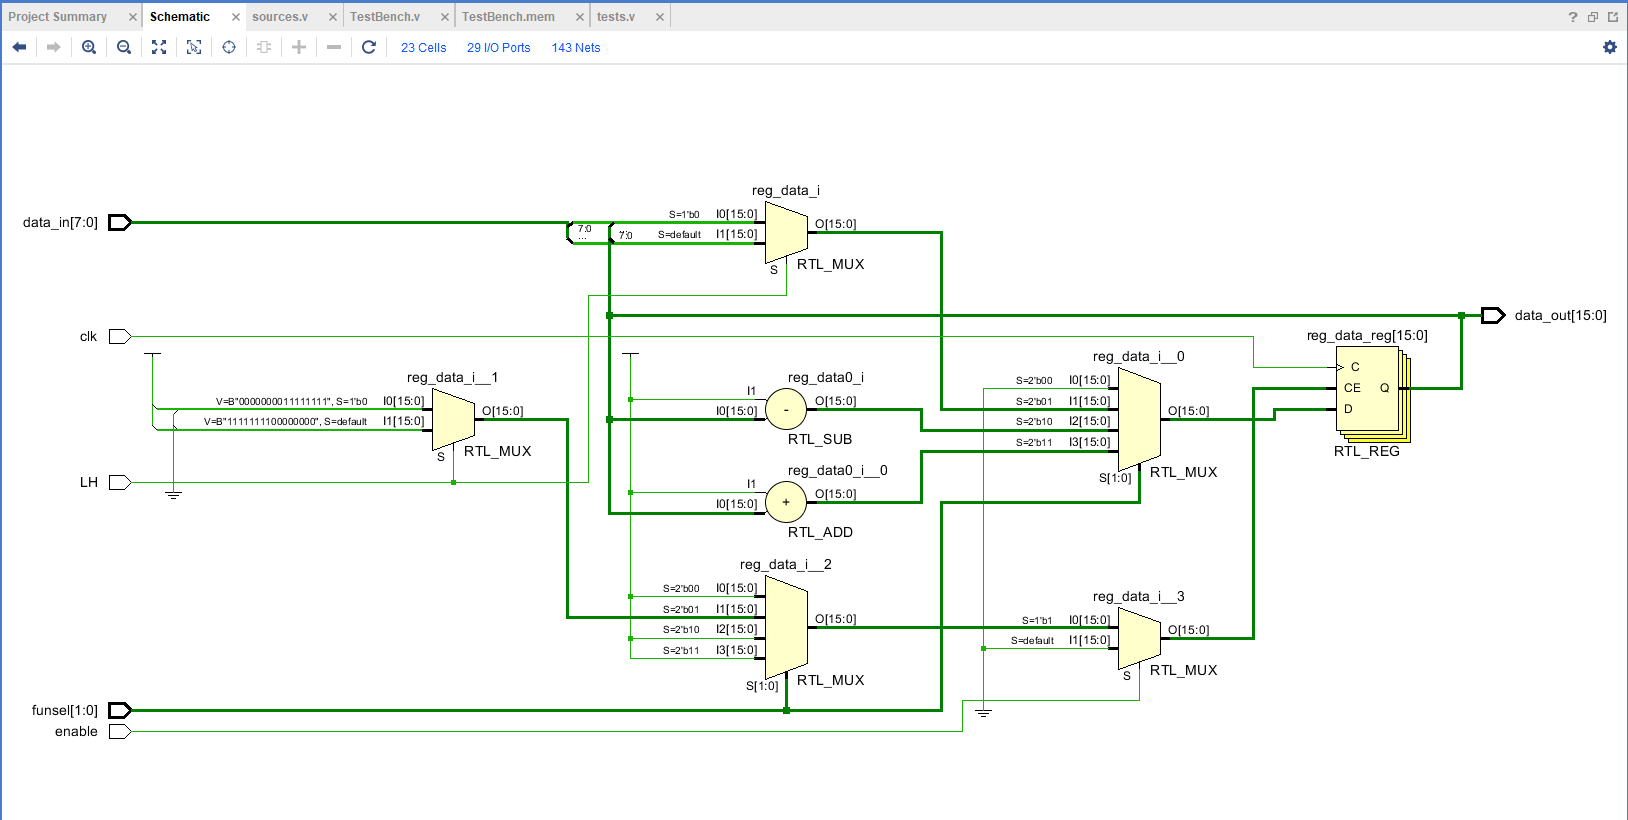
\includegraphics[width=1\textwidth]{Project1/Design Photos/IR_16.png}	
	\caption{16-Bit Register RTL}
	\label{figthree}
\end{figure}

\begin{figure}[H]
	\centering
	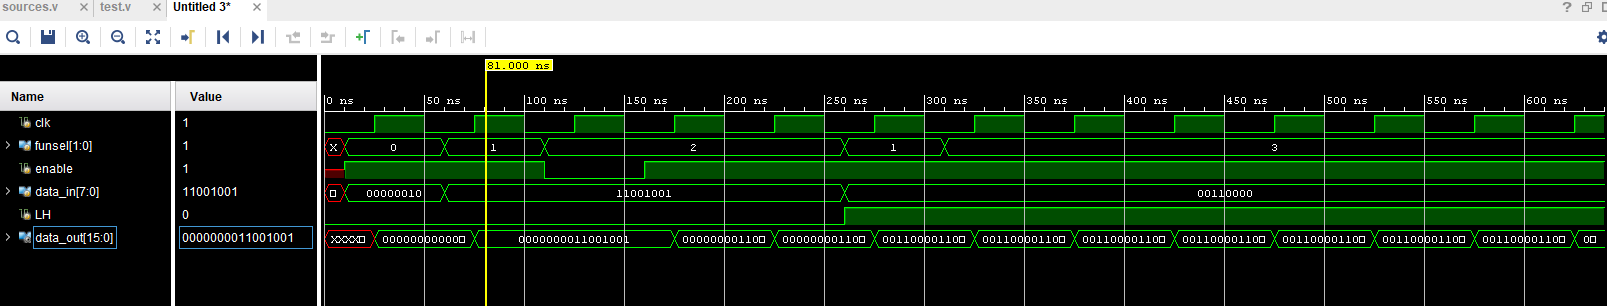
\includegraphics[width=1\textwidth]{Project1/Test Photos/IR_16_binary_test.png}	
	\caption{16-Bit Register Simulation}
	\label{figfour}
\end{figure}


\subsubsection{PART 2.B}
Using general purpose and temporary registers,  we built a system that takes inputs such as O1Sel, O2Sel, FunSel, RSel, and TSel; gives outputs as O1 and O2 with n-bit registers that we implemented in the first part.

\begin{figure}[H]
	\centering
	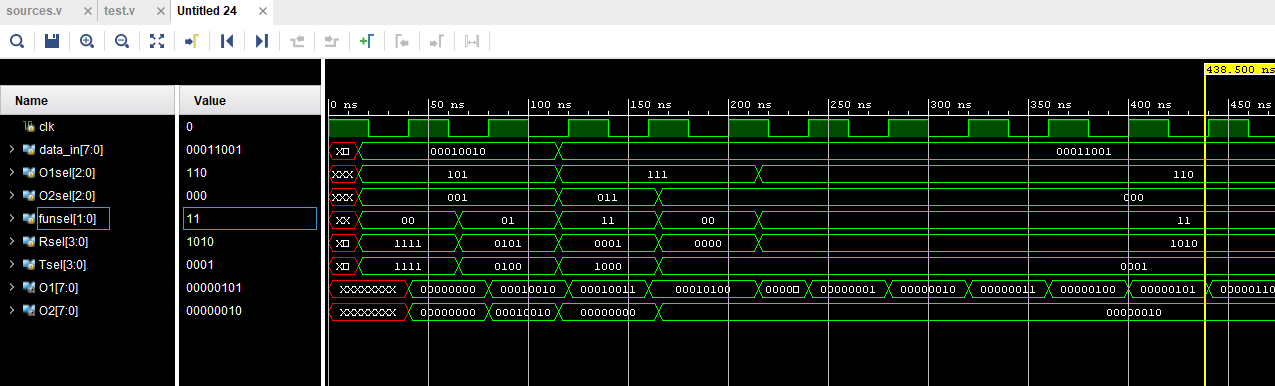
\includegraphics[width=1.10\textwidth]{Project1/Test Photos/part2b_test.png}	
	\caption{Register File Simulation}
	\label{figfive}
\end{figure}


\begin{figure}[H]
	\centering
	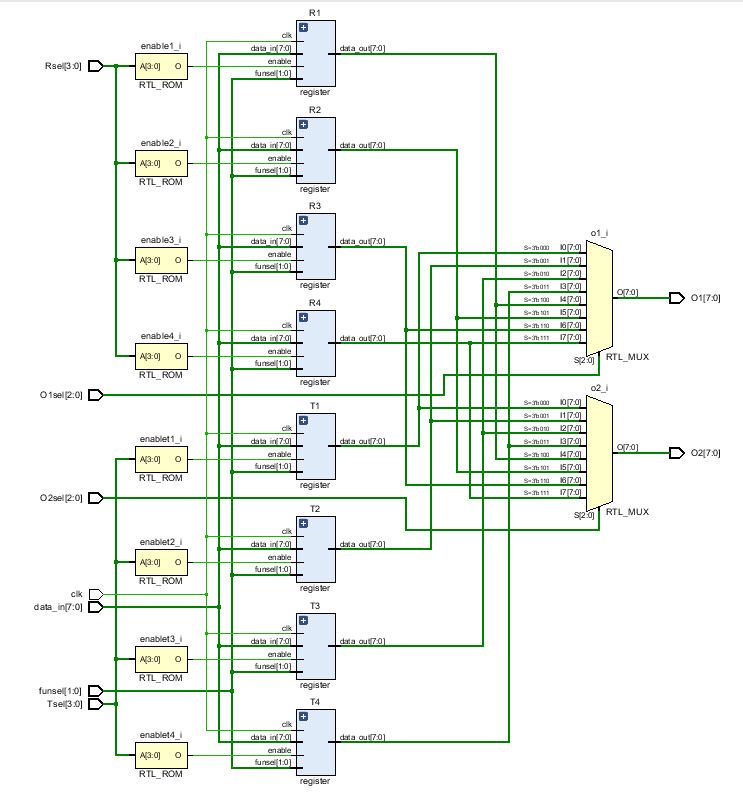
\includegraphics[width=1.15\textwidth]{Project1/Design Photos/part2b.png}	
	\caption{Register File RTL}
	\label{figsix}
\end{figure}



\subsubsection{PART 2.C}
We have designed the address register file in this section which includes the program counter (PC), address register (AR), stack pointer (SP), and the past program counter (PCPast). This system takes inputs as OutASel, OutBSel, FunSel, and RSel; gives outputs as OutA and OutB.

\begin{figure}[H]
	\centering
	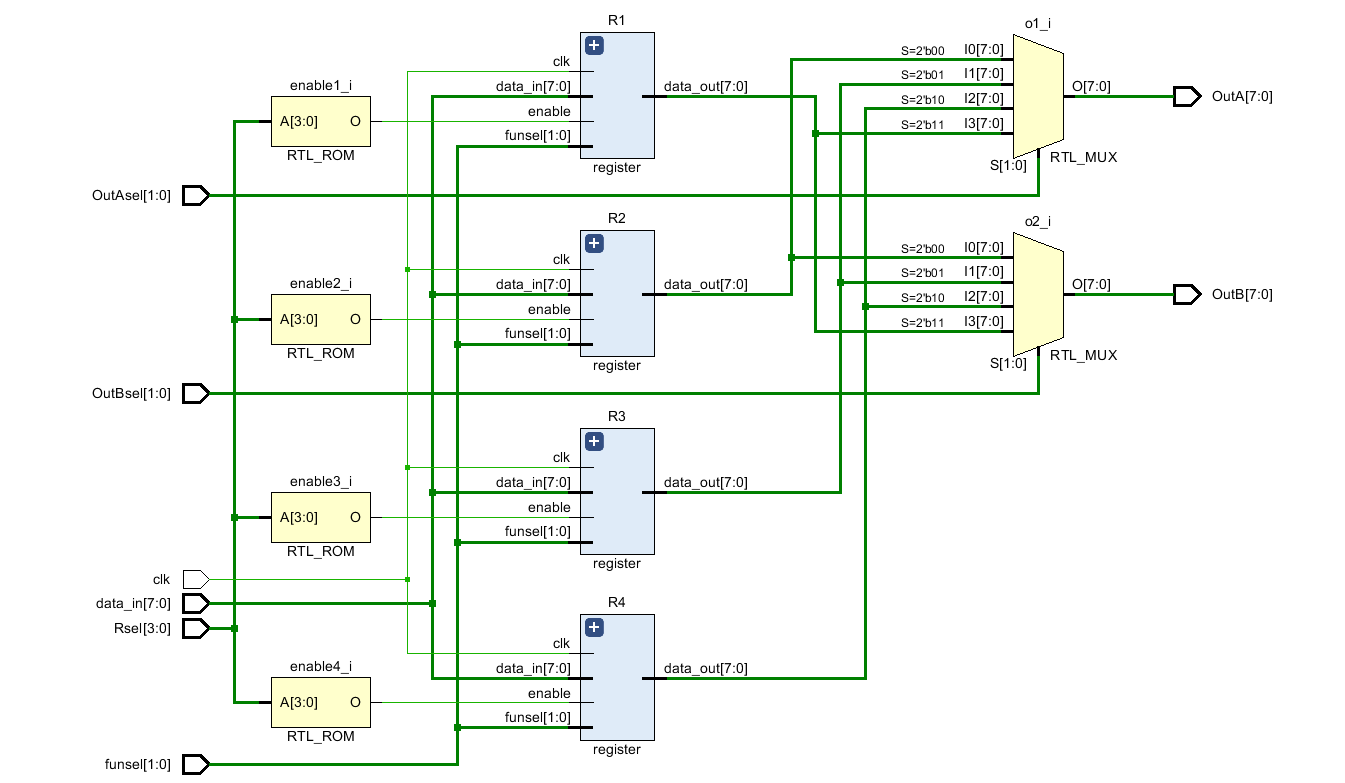
\includegraphics[width=1\textwidth]{Project1/Design Photos/part2c.png}	
	\caption{Address Register File RTL}
	\label{fig1}
\end{figure}

\begin{figure}[H]
	\centering
	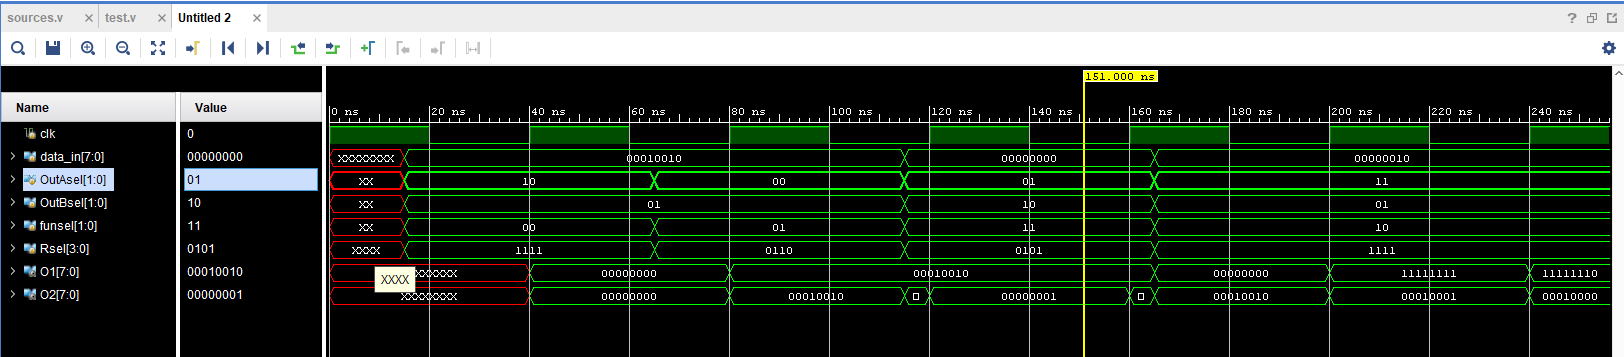
\includegraphics[width=1\textwidth]{Project1/Test Photos/part2c_test.png}	
	\caption{Adress Register File Simulation}
	\label{figeight}
\end{figure}


\subsection{PART 3}
We have implemented an ALU using FunSel as input which leads to complement, addition, subtraction, AND, OR, NAND, XOR, compare, and shifting operations. This module gives output as OutALU and there is a register that specifies Z (zero), C (carry), N (negative), and O (overflow) flags.

\begin{figure}[H]
	\centering
	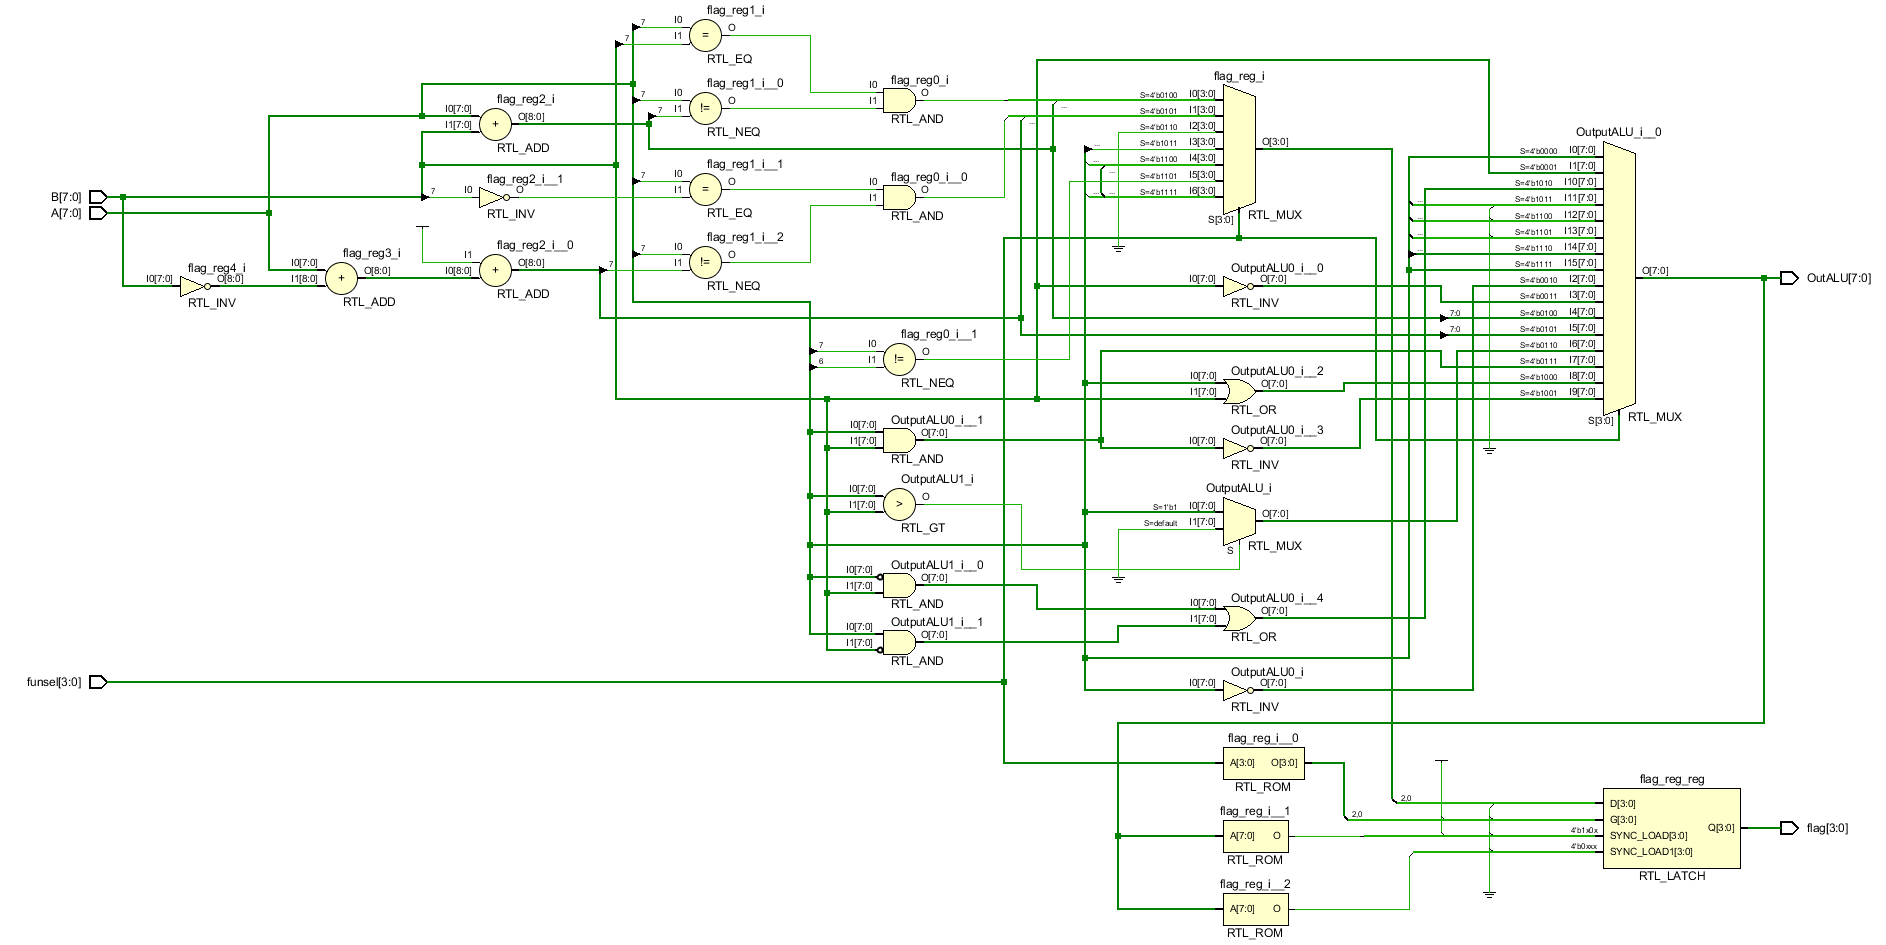
\includegraphics[width=1\textwidth]{Project1/Design Photos/part3_ALU.png}	
	\caption{ALU RTL}
	\label{fignine}
\end{figure}

\begin{figure}[H]
	\centering
	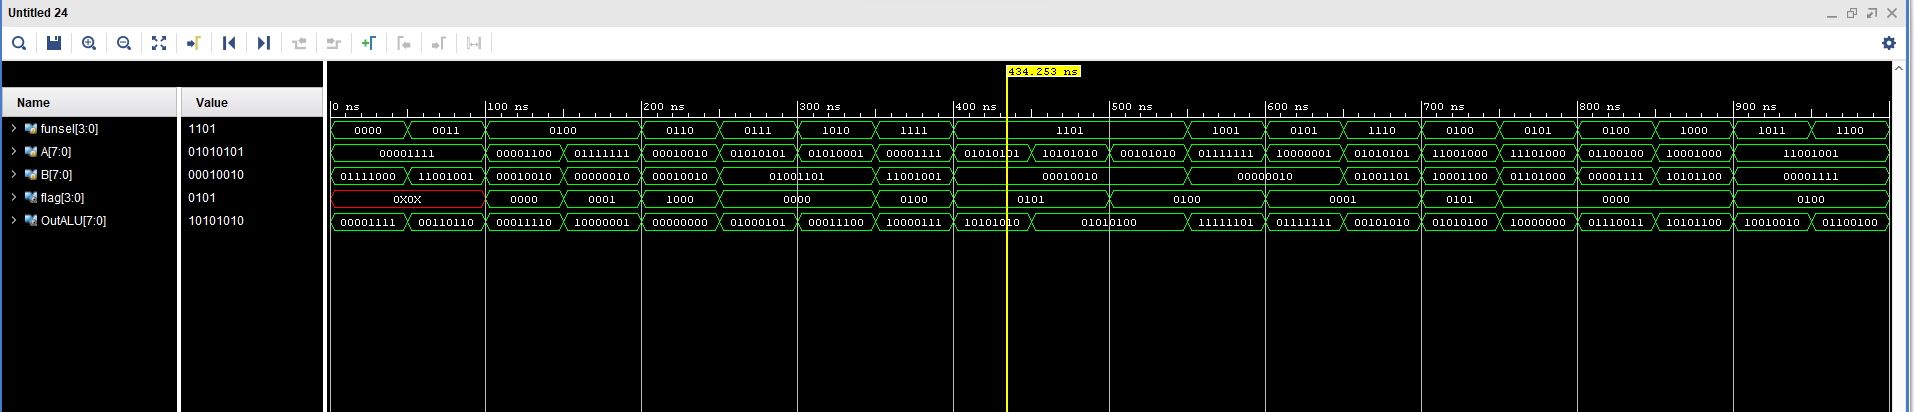
\includegraphics[width=1\textwidth]{Project1/Test Photos/part3_ALU_test.png}	
	\caption{ALU Simulation}
	\label{figten}
\end{figure}


\subsection{PART 4}
In this part, previous parts have been integrated with three multiplexers to build a whole ALU system that uses a single clock signal. RAM module and memory data have been added to the project.

\begin{figure}[H]
	\centering
	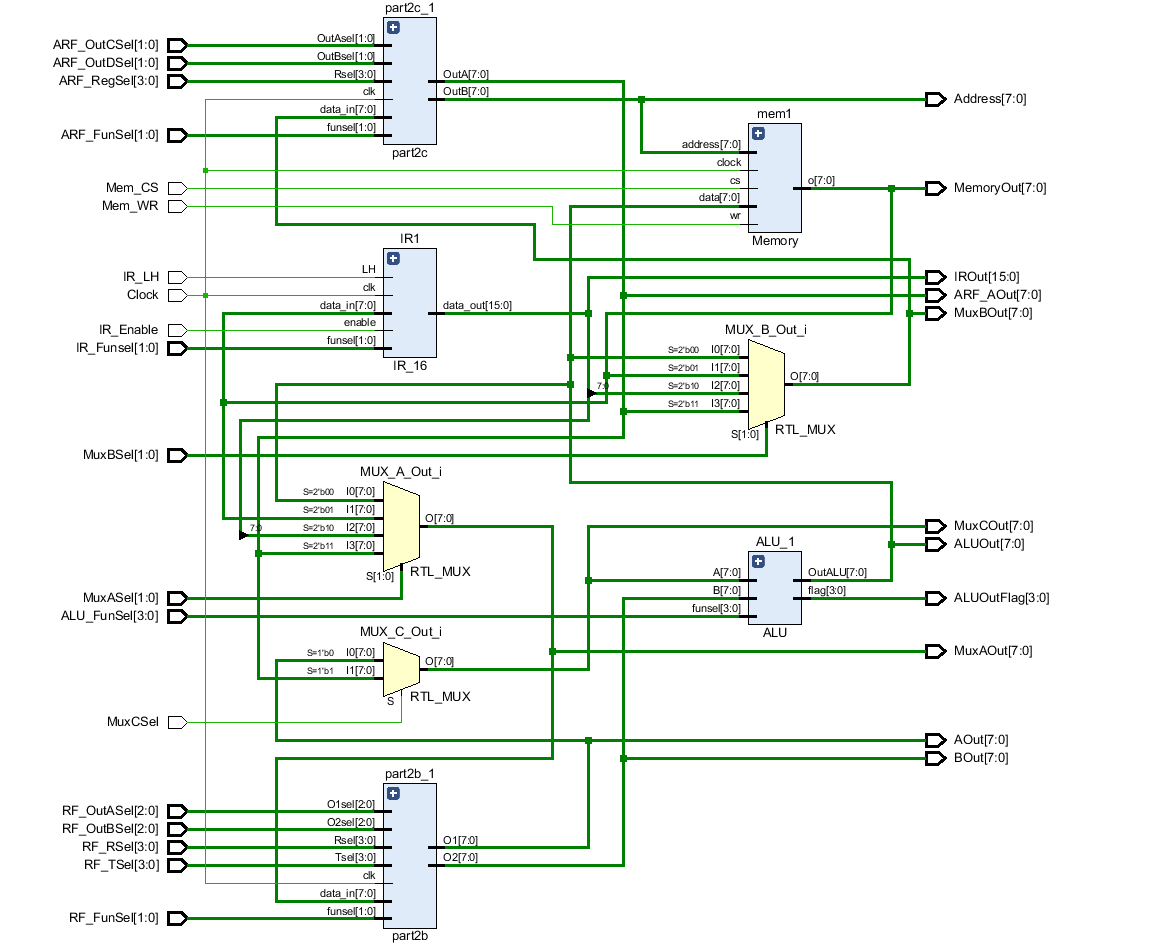
\includegraphics[width=1\textwidth]{Project1/Design Photos/part4_ALU_System.png}	
	\caption{ALU System RTL}
	\label{figeleven}
\end{figure}

\begin{figure}[H]
	\centering
	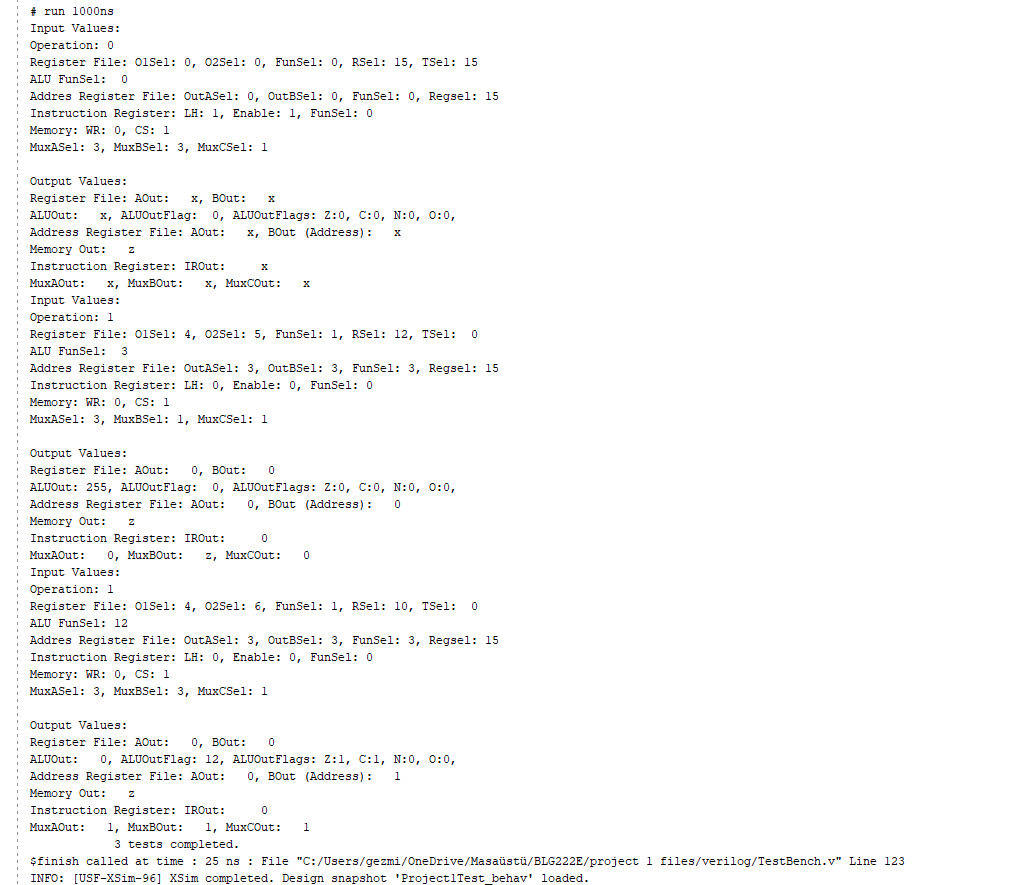
\includegraphics[width=1\textwidth]{Project1/Test Photos/ALU_system_output.png}	
	\caption{ALU System Terminal Messages}
	\label{figtwelve}
\end{figure}

\begin{figure}[H]
	\centering
	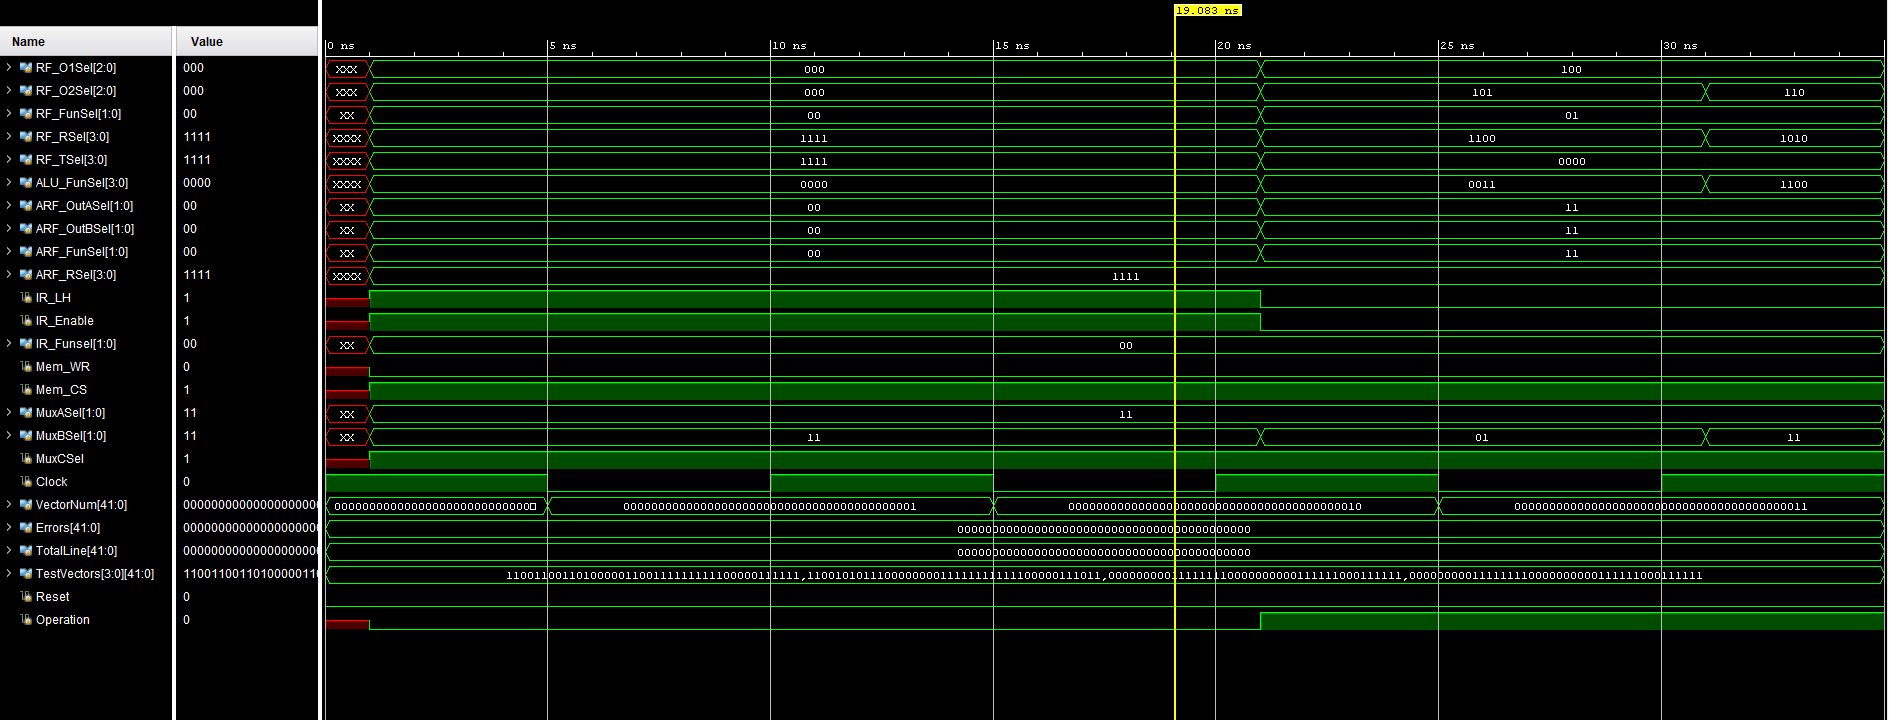
\includegraphics[width=1\textwidth]{Project1/Test Photos/ALU_system_tb.png}	
	\caption{ALU System Simulation}
	\label{figthirteen}
\end{figure}



\section{RESULTS}
We have experienced that by using registers, we can obtain the ALU system, thus; the working principle of the logic and arithmetic operations performed by digital circuit components has been understood clearly.


\section{DISCUSSION}
Firstly,  we analyzed the project as a group and decided what our steps needs to be to create our ALU project. We divided our work into parts. However, after a while, we figured out that working on parts separately will be more stressful and difficult due to preparing the parts and include to each other, etc. After that, we worked together on the parts. We created the logic designs and write Verilog codes cooperatively for all the parts. We had difficulties from time to time while we trying to understand registers and the systems, but eventually, we analyzed correctly. We finished our project early before the due time. However, we waited for the test-bench typos to be resolved.

\section{CONCLUSION}
In this project, firstly; we have built an n-bit register and used it to create an instruction register (IR), general purpose, and temporary registers. Then, we used it for implementing an address register file including different types of registers such as program counter (PC), address register (AR), stack pointer (SP), and the past program counter (PCPast). Finally, using these parts, Arithmetic Logic Unit has been implemented and after the organization of the system, the performance of the whole system has been observed with the same clock signal.

\newpage
\addcontentsline{toc}{section}{\numberline {}REFERENCES}

\bibliographystyle{unsrt}
\bibliography{reference}

\end{document}

